% Ubah judul dan label berikut sesuai dengan yang diinginkan.
\section{Cyclic Redundancy Check}
\label{sec:crc}

% Ubah paragraf-paragraf pada bagian ini sesuai dengan yang diinginkan.

% % Contoh input beberapa gambar pada halaman.
% \begin{figure*}
%   \centering
%   \subfloat[Hasil A]{\includegraphics[width=.4\textwidth]{example-image-a}
%     \label{fig:hasila}}
%   \hfil
%   \subfloat[Hasil B]{\includegraphics[width=.4\textwidth]{example-image-b}
%     \label{fig:hasilb}}
%   \caption{Contoh input beberapa gambar.}
%   \label{fig:hasil}
% \end{figure*}

Sebuah \emph{Cyclic Redundancy Check} adalah \emph{error-detecting code} yang biasa digunakan pada jaringan digital dan storage untuk mendeteksi adanya perubahan yang tidak diinginkan pada data. Blok data yang memasuki sistem CRC akan diberikan \emph{check value}, berdasarkan sisa dari pembagian polinomial dari kontennya. Saat pengambilan data, kalkulasi tersebut diulang lagi dan apabila check value tidak sesuai maka dapat dilakukan koreksi untuk menghindari data yang korup. CRC dapat digunakan untuk \emph{error-correction} \citep{dobbs2003}. Varian CRC-1 dikenal juga sebagai parity bit (\ref{sec:paritybit}).

Sejatinya, CRC merupakan tipe dari checksum, dan memiliki konsep yang mirip dengan checksum. Akan tetapi, terdapat perbedaan diantaranya sehingga saya memutuskan untuk memberikannya bab tersendiri. CRC merupakan checksum yang secara spesifik adalah \emph{position dependent checksum algorithm}. Dari namanya tersebut, CRC dapat mendeteksi perpindahan posisi, yang membuatnya menjadi integrity check yang umum digunakan. CRC juga populer dikarenakan kesederhanaannya dibandingkan algoritma checksum yang lainnya seperti MD5 dan SHA family. CRC juga lebih mudah untuk dianalisis secara matematis dan baik untuk mendeteksi error yang umum terjadi dikarenakan oleh noise pada transmission channel. CRC sendiri tidak didesain dengan tujuan kriptografik, karena CRC dapat direverse sehingga untuk alasan keamanan lebih dianjurkan untuk menggunakan SHA-2. CRC biasa digunakan dalam hal untuk menyalin atau memindahkan file serta kompres dan dekompres file.

\subsection{Integritas Data}
\label{subsec:crcdataintegrity}

Seperti yang sudah disebutkan sebelumnya, CRC didesain secara spesifik untuk keperluan error-checking, dimana CRC akan mendeteksi kesalahan dengan beban komputasi yang jauh lebih ringan dibandingkan dengan Cryptographic Hash Function. Maka dari itu, CRC tidak cocok untuk melindungi dari modifikasi data yang disengaja. Yang pertama, karena tidak ada autentikasi, \emph{attacker} dapat memodifikasi pesan dan menghitung ulang CRCnya tanpa terdeteksi. Ketika disimpan bersama dengan data, baik CRC maupun Cryptographic Hash Function tidak melindungi dari perubahan data yang disengaja. Aplikasi yang memerlukan proteksi dari serangan tersebut harus menggunakan mekanisme autentikasi kriptografik, seperti \emph{message authentication codes} (MAC) atau \emph{digital signatures}. Yang kedua, tidak seperti MD5 maupun SHA, CRC dapat dengan mudah direverse, yang membuat CRC tidak cocok untuk digunakan sebagai \emph{digital signatures} \citep{martin2006}. Yang ketiga, CRC memiliki hubungan yang mirip dengan fungsi linear \citep{poncho2016}. 

\begin{equation}
  \label{eq:crc1}
  CRC(x\oplus y) = CRC(x) \oplus CRC(y) \oplus c
\end{equation}

Dimana \(c\) bergantung dari panjang \(x\) dan \(y\). Persamaan \ref{eq:crc1} juga bisa dituliskan seperti berikut, dimana \(x\), \(y\), dan \(z\) memiliki panjang yang sama.

\begin{equation}
  \label{eq:crc2}
  CRC(x\oplus y \oplus z) = CRC(x) \oplus CRC(y) \oplus CRC(z)
\end{equation}

Maka, bahkan ketika CRC dienkripsi dengan \emph{stream cipher} yang menggunakan XOR sebagai operasi kombinasinya, baik pesan maupun CRC dapat dimanipulasi tanpa sepengetahuan dari \emph{encryption key}, ini merupakan salah satu \emph{design flaws} dari protokol Wired Equivalent Privacy (WEP) \citep{winget2003}.

\subsection{Algoritma}
\label{subsec:crcalgorithm}

Komputasi dari CRC diturunkan dari polynomial division, modulo dua. Ini menyerupai pembagian dari pesan string biner, dengan nol bit yang jumlahnya tetap diappend oleh string "generator polynomial", tetapi dengan menggunakan XOR, bukan pengurangan. Pembagian jenis ini sudah direalisasikan di harware dengan shift register yang sudah dimodifikasi \citep{dubrova2012}. Contoh dari implementasi polynomial division pada hardware, misalnya kita mencoba untuk menghitung CRC 8-bit dari pesan 8-bit yang terdiri dari karakter ASCII "W", yang binernya adalah \(01010111_2\), desimal \(87_10\) atau hexadecimal \(57_16\). Sebagai ilustrasi, kita menggunakan CRC-8-ATM (HEC) polinomial \(x^6+x^2+x+1\). Menuliskan bit pertama yang ditransmisikan (koefisien dari pangkat tertinggi \(x\)) di sebelah kiri, sesuai dengan string 9-bit "100000111". Nilai byte \(57_16\) dapat dikirimkan dalam dua urutan berbeda, bergantung dari konvensi urutan bit yang digunakan. Tiap urutan menghasilkan pesan polinomial \(M(x)\) yang berbeda. Msbit-first, \(x^6+x^4+x^2+x+1\) = 01010111, bila lsbit-first, \(x^7+x^6+x^5+3+1\) = 11101010. Nilai ini dapat dikalikan dengan \(x^8\) untuk menghasilkan dua pesan 16-bit polinomial \(x^8M(x)\). Menghitung sisanya terdiri dari mengurangi kelipatan dari generator polinomial \(G(x)\). Ini hanya seperti pembagian desimal, tapi lebih sederhana karena kelipatan yang mungkin hanyalah 0 dan 1, dan pengurangannya meminjam dari "tak terhingga", bukan mengurangi dari digit yang lebih tinggi. Karena kita tidak peduli dengan hasil bagi, maka tidak perlu dituliskan.

\begin{figure} [ht]
  \centering
  % Ubah sesuai dengan nama file gambar dan ukuran yang akan digunakan.
  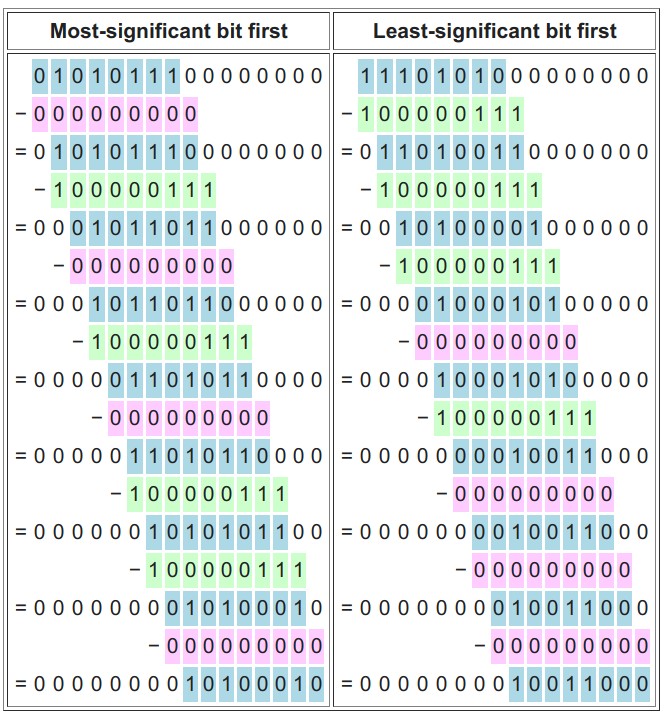
\includegraphics[width=0.4\textwidth]{gambar/komputasicrc.png}

  % Ubah sesuai dengan keterangan gambar yang diinginkan.
  \caption{Perhitungan polynomial division}
  \label{fig:crccomputation}
\end{figure}

Perhatikan bahwa untuk setiap pengurangan, bit-bitnya dibagi menjadi 3 bagian, grup yang berisi nol, grup yang tidak diubah dari originalnya, dan grup yang berwarna biru, yang "menarik". Grup yang menarik ini panjangnya 8-bit, menyamai pangkat dari polinomial. Setiap langkah, kelipatan yang benar dikurangi untuk membuat grup nol menjadi satu bit lebih besar, dan grup yang tidak berubah menjadi satu bit lebih pendek, hingga akhirnya meninggalkan satu sisa.

% Contoh input potongan kode dari file.
\lstinputlisting[
  language=Python,
  caption={Program CRC.},
  label={lst:crccomputation}
]{program/crccomputation.py}

Program dari listing \ref{lst:crccomputation} berisi fungsi yang akan mereturn nilai sisa awal dari CRC untuk input dan polinomial yang ditentukan, entah dengan 1 atau 0 sebagai padding awalnya.

\begin{lstlisting}[
  language=Python,
  caption={Output dari listing \ref{lst:crccomputation}.},
  label={lst:outputcrc}
]
>>> crc_remainder('11010011101100', '1011', '0')
'100'
>>> crc_check('11010011101100', '1011', '100')
True
\end{lstlisting}

\lstinputlisting[
  language=C,
  caption={Program CRC dalam bahasa C.},
  label={lst:crcwithc}
]{program/crc.c}

Listing \ref{lst:crcwithc} merupakan algoritma CRC-32 \citep{microsoft2019} dalam bahasa C. Variable \lstinline{CRCTable} adalah memoization dari kalkulasi yang harus diulang untuk setiap byte dari pesan.

\subsection{Kompresi Data}
\label{subsec:kompresidata}

CRC digunakan untuk melakukan kalkulasi dari semua data yang ada di dalam file yang terkompresi. Nilai CRC akan dikalkulasi setiap kali ada file baru yang ditambahkan kedalam archive. Ketika archive atau file terkompresi di dekompresi, maka program akan mengkalkulasi nilai CRC kembali dan membandingkannya dengan yang ada di archive. Apabila terdapat perbedaan pada CRC value, maka biasanya akan ditampilkan pesan CRC error, yang mengindikasikan bahwa file yang terekstrak tidak sama dengan file yang awalnya dikompresi. Hal ini biasanya terjadi ketika file yang dikompresi didalam archive rusak. Hal ini juga dapat terjadi walaupun hanya satu file didalam archive yang korup.

Nilai dari CRC itu sendiri tidak mengatakan bahwa file anda korup atau tidak. Maka, ketika kita mengecek metadata dari archive atau mengkompresi file dan menemukan nilai CRC-nya, bukan berarti archive kita telah rusak. Hal tersebut hanya menunjukkan nilai awal dari CRC file yang terkompresi. Kebanyakan software untuk melakukan kompresi seperti 7zip dan WinRAR sudah memiliki mekanisme ini \citep{7zip}.
